\chapter{Requirements Analysis and Specification}

After a short introduction to the basic terms and Apache Flink and Apache Kafka in
context of stream processing, this chapter examines what different kind of data are available
for both of the systems. According to the results of the data analysis, the functional and
non-functional requirements of the software system which is forming the core of the present
thesis will be defined.

\section{Data Analysis}

In preparation of this thesis my supervisor Prof. Dr. Stefan Edlich once said \textit{"Sie sammeln
alles, was nicht bei drei auf dem Baum ist"}. According to this statement, the main focus
of the coming section is the analysis of available data that will be collected by the software
solution and not a deeper exploration according to the relevance and quality of data that
is available for Apache Flink and Apache Kafka.

\textit{"You can only control what you observe and measure."}\cite{Ebert07}. Even though logfiles, both
provided by Apache Flink and Apache Kafka, are usefull for tracing problems in software
systems, problems can be tracked and potential sources of error can be identified much
earlier by collecting and storing system and application data at runtime to describe the
state of the entire system at a given point in time.

Due to the distributed character of Apache Flink and Apache Kafka, where a system is
composed of several interacting components, the examination of log data is not an
adequate choice to gain insight into a distributed system containing several components.\cite{VanL14}.

Runtime data to collect can be divided in three levels of abstraction:

\begin{enumerate}
    \item \textbf{Business data:} The highest level of abstraction, often refered to as Key Performance
    Indicators(KPI), these data expresses direct business related values and
    usually have very little reference to technical details. As an example, the number of
    sales in an online shop.
    \item \textbf{Application data:} On the middle level of abstraction, application data already
    contains many more technical details and refers to specific applications, like the
    number of GET requests and their corresponding HTTP Status response codes of a
    REST-based service.
    \item \textbf{System data:} The lowest level of abstraction, data provided by the underlying
    systems an application is running on such as cpu, memory, network, or system utilization.
\end{enumerate}

Based on Apache Flink and Apache Kafka, the following section discusses the data provided
by both of the systems and tries a classification based on the abtraction levels.

\subsection{System data}

System data refers to the data provided by the computer system on the lowest level of
abstraction and allows observation of system-related data. On unix-based systems, a
variety of system tools is well known to system administrators to monitor the performance
of servers, like vmstat (memory utilization), ifstat (network usage) or iostat (system
input/output) \cite{Hoeb12}.

Another existing tool is called "DStat Versatile Resource Statistics Tool" and is described
as follows: \textit{"Dstat is a versatile replacement for vmstat, iostat, netstat and ifstat. Dstat
overcomes some of their limitations and adds some extra features, more counters and flexibility.
Dstat is handy for monitoring systems during performance tuning tests, benchmarks
or troubleshooting. Dstat allows you to view all of your system resources in real-time, you
can eg. compare disk utilization in combination with interrupts from your IDE controller,
or compare the network bandwidth numbers directly with the disk throughput (in the same
interval)."}\cite{Wieers16}

Dstat is a command line tool, the following figure shows the immediate output of running
the application with the argument "--full", which expands more detailed information about
multiple cpus and network interfaces:

\begin{figure}[H]
	\centering
	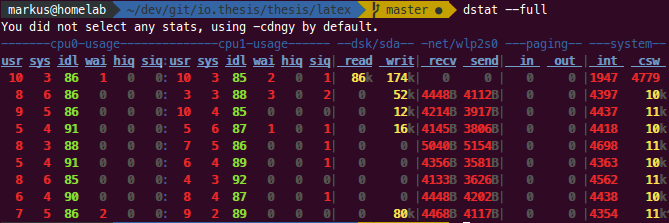
\includegraphics[width=1.0\textwidth]{../images/06-dstat-full.png}
	\caption{Output "dstat --full"}
	\label{dstat-output}
\end{figure}

Additionally, Dstat provides multiple parameters to specify the data to be displayed, e.g.
--cpu, --disk, --net, and many more. Used in combination, the data can be grouped in the
following categories according to the parameters:

\begin{table}[H]
    \begin{tabular}{ll}
        \textbf{Category} & \textbf{Dstat parameters} \\
        cpu & ("--cpu", "--top-cpu-adv", "--top-cputime", "--top-cputime-avg")\\
        disk & ("--disk", "--disk-tps", "--disk-util")\\
        net & ("--net", "--socket", "--tcp", "--udp")\\
        io & ("--io", "--top-io-adv", "--lock", "--fs")\\
        memory & ("--mem", "--top-mem", "--page", "--swap", "--vm")\\
        system & ("--sys", "--load", "--ipc", "--unix")\\
        process & ("--proc", "--proc-count", "--top-latency", "--top-latency-avg")\\
    \end{tabular}
    \caption{Dstat data categories}
    \label{tbl:dstatcategories}
\end{table}

Although the parameters are mostly self-explanatory, a list containing short descriptions
for each of the parameter used in Chapter 4 Architecture and Implementation is available in
Appendix. TODO Based on the data in the extracted categories, Dstat can be considered
as a source that gives a fairly complete picture of the state of a system.

Dstat is a tool only available for unix systems, and therefore not available for Windows or
Macintosh. Since Apache Flink and Apache Kafka are operated on Unix systems in most
cases, this fact can be neglected because this tool offers a wide range of data to describe
the system state a certain point of time.


%What to Transport? Logs vs. Metrics see http://blog.mmlac.com/log-transport-with-apache-kafka/
%The first consideration should be if it is possible and/or necessary to transport all logs to a central
%location. If there are many servers or a lot of log data, this might be very resource intensive and aggregating
%or filtering the data might be necessary. The extremes of this are either transporting every single log vs. only
%transporting aggregated metrics. The following paragraphs try to help you decide on the right balance for your use case.
%
%Advantages of transporting all logs:
%
%Metrics can be added, modified and deleted in one central location
%Historical data on new metrics can be computed from the stored logs
%Possibility to peek into live data-stream
%Allows building complex debugging and monitoring tools
%Central location for all logs. Invaluable for debugging, root-cause analysis and correlation of incidents
%Advantages of transporting only metrics:
%
%Transporting (aggregated) metrics requires far less bandwidth
%Smaller storage requirements
%Scales far better
%Better than nothing
%Overall transporting all logs has many advantages and should be preferred over aggregated metrics if possible. Especially managing metric definitions in one place and the ability to compute historic data for new metrics is very valuable. Also does transporting all logs allow for thorough (computationally expensive) data analysis on historic data to i.e. train machine learning models, predict behavior or give enhanced insights into who your users are and what they do.
%
%There is no strict rule to follow and it is perfectly ok to mix and match. An example would be to just transport logs that contain examinable data and aggregate performance metrics, like average response time or jobs processed per minute, on the server.
%
%This post will focus on the transport of raw log data. The posts “Server Monitoring with Sensu” and “Metrics with Graphite” will introduce better suited technologies to work with pure metrics.
\subsection{Application data}

Every application running on the Java Virtual Machine, can be accessed via JMX as discussed
in Chapter 2 Basic Concepts. According the specification, every implementation of the JVM contains
implementations for a basic set of management interfaces, that enables the access separate parts of JVM related data,
located in the package "java.lang.management" \cite{Javadoc16}.

\begin{table}[H]
    \begin{tabular}{ll}
        \textbf{Management interface} & \textbf{JMX ObjectName} \\
        ClassLoadingMXBean & java.lang:type=ClassLoading \\
        OperatingSystemMXBean & java.lang:type=OperatingSystem \\
        RuntimeMXBean & java.lang:type=Runtime \\
        ThreadMXBean & java.lang:type=Threading \\
        MemoryMXBean & java.lang:type=Memory \\
        BufferPoolMXBean & java.nio:type=BufferPool,name=* \\
        GarbageCollectorMXBean & java.lang:type=GarbageCollector,name=* \\
        MemoryManagerMXBean & java.lang:type=MemoryManager,name=* \\
        MemoryPoolMXBean & java.lang:type=MemoryPool,name=* \\
    \end{tabular}
    \caption{"Default" JMX JVM data}
    \label{tbl:jmxjvmdata}
\end{table}

There's a difference in the way of data access between the object name containing an asterisk "*"
and the one the ones that doesn't. The asterisk indicates the existence of multiple MBeans for a given query string,
the result of a query for the object name "java.lang:type=GarbageCollector,name=*" results in multiple data sets according
to existing garbage collector names.

This "default" set of management interfaces provides a deep insight into JVM data, is
available for Apache Flink and Apache Kafka and will be included in the software solution
in Chapter 4.

In addition to the standard interfaces and MBeans that come with the implementation of the JVM,
Apache Kafka provides a set of managed resources providing application specific
metrics concerning the Kafka domain, reaching from global broker metrics, global connection metrics to
metrics per topic like in- and outgoing byte rates for example. Based on the requirement to collect as
much data as possible, the data of all provided resources will be collected, the complete list of MBeans observed
for Apache Kafka is available in Appendix A.

TODO: Apache Flink provides application data via Monitoring REST API, since version 1.1.0 new Metrics data via JMX.

According to these examinations, the following matrix of data sources results for Apache Flink and Apache Kafka:

\begin{table}[H]
%\centering
\begin{tabular}{lllll}
 & System data (Dstat) & "Default" JVM data & AD JMX & AD REST \\
Apache Flink & X & X & X & X \\
Apache Kafka & X & X & X & - \\
\end{tabular}
\caption{Data source matrix, AD=application data}
\label{data-source-matrix}
\end{table}

TODO: Correlation sytem and application data
%
%\section{Data Quality}
%
%Define DQ, evaluate quality for data above

\section{Functional Requirements}
see Main goal, ased on the data analysis,...TODO
%Collect DStat system data
%Collect JVM data for Apache Flink and Apache Kafka
%Collect
%
%
%
%
%The main objective of this bachelor thesis is to implement a software solution to collect ....
%"COLLECT EVERYTHING!
%live and historical sources
%
%Describe "big picture" functionality see \cite{VanL14}, follows distributed character of Big Data Analytics
%Applications, provide "on demand" data collection, as much data as possible, realtime?, three main components,
%break down for:
\subsection{Collection}
%collect data in clustered environments

\subsection{Transport}
%Scalability with message broker

\subsection{Persistence}
%Accessibility for AI, UI applications

\section{Non-Functional Requirements}
%Performance, scalability,
%simplicity, modifiability, visibility, portability, and reliability

\section{Summary}